
\chapter{Business Rules}

Businesses are run in terms of various types of information. This
includes resource information, marketing strategies, customer information,
etc. A key part of the information underlying a business are the policies
by which the business operates. Policies are the guidelines by which
all components of the business are co-ordinated. Policies are used
to determine what happens when various events take place within the
business. Events include day-to-day occurrences such as new customer
contact, and also include longer term strategic events such as a company
merger or implementing a new product.

Often the rules that drive a business are left implicit within the
structure of the organisation. Some of the rules may be written down
in company literature (such as an employee handbook) and others may
simply be in the heads of individuals. There is significant advantage
in producing a complete collection of the rules that drive a business.
Once the rules are brought together in a uniform representation they
can be analysed in terms of their impact on the business. 

Representing the rules as executable models has added benefit: the
rules can be used to simulate the business in different scenarios.
By executing the business in terms of its models, it is possible to
try out different strategies and to get a feel for the effect of changes
to how the business operates. Furthermore, it may be possible to run
certain parts of the business directly from the executable business
rules; changes to the strategy can then be implemented directly by
changing the rules.

Typically, business rule systems are event driven. The rules monitor
business data; changes to the business data are detected as events
by the rules which in turn fire actions that update the business data.
For example, rules may monitor an invoice database; an event is raised
when an invoice is received from a customer causing the rule to fire
and an email to the appropriate sales manager is sent.

A rules engine must manage large collections of rules that monitor
events across a very large amount of business information. A naive
implementation of a business rules engine might run all rules against
all the business data each time an event occurs. This is far too expensive
because of the speed of change in many businesses and the combinations
of data that must be checked. 

Fortunately, the problem has been solved by a special type of matching
algorithm called the Rete Algorithm that uses caching of partial matches
to produce huge reductions in the amount of retesting required by
a rule engine each time the data changes. This chapter describes how
to develop language constructs for business rules and to implement
a business rule engine using XOCL.


\section{Example Business Rules}

%
\begin{figure}
\begin{center}

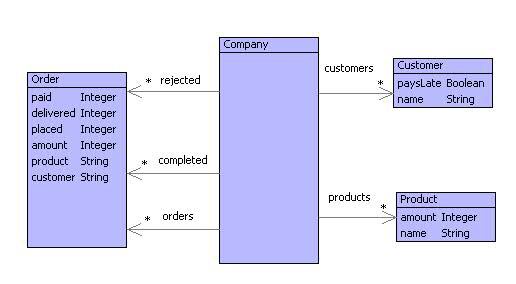
\includegraphics[width=12cm]{LanguageEngineering/BizRules/Images/Companies}

\caption{A Sales Order Information Model\label{fig:A-Sales-Order}}

\end{center}
\end{figure}


Consider the sales order information model shown in figure \ref{fig:A-Sales-Order}.
This is part of a larger information model that is used to represent
the state of a company at any moment in time. Customers initially
contact the company with a sales order for a named product. If the
customer does not already exist then they are added to the customers
database. The order is then analysed to determine whether it can be
met. An order can only be processed if the company has sufficient
amount of the required product. If the order cannot be met then it
is placed in the rejected orders database and the customer is informed
by letter. 

The order may also be rejected if the customer pais late. The company
has a policy that requires payment for an order to be received within
30 days of the order being received. If the customer fail to satisfy
this policy then they become marked and all subsequent orders are
rejected until appropriate representations are made to senior management.

Once an order has been received and accepted, the product is packaged
up and sent to the customer. On dispatching the goods, the order is
moved to the completed orders database.

The order system described above includes an number of policies that
can be expressed using business rules. Business rules are grouped
into business aspects, the sales order processing system is such an
aspect:

\begin{lstlisting}
@RuleBase OrderProcessing
  // Business Rules...
end
\end{lstlisting}Each major policy that is used to drive the business is expressed
as a rule. The following rule describes what happens when an order
is received:

\begin{lstlisting}
context OrderProcessing
(1)  @Rule ReceiveOrder
(2)    Company[c]
(3)    Order[o]
(4)    ? not c.hasOrder(o) end
(5)  -> 
(6)    c.addToOrders(o)
     end
\end{lstlisting}The rule named ReceiveOrder is defined in line (1). It has a head
(lines (2) - (4)) and a body (line(6)). The head of the rule describes
a situation that may occur in the business. ReceieveOrder describes
a situation where an order is received by the business but has not
yet been entered into the orders database. Line (2) detects any company
and associates the variable c with the company. Line (3) detects any
order and associates variable o with it. Line (4) is a general condition
that can be any XOCL expression using any of the variables in scope.

The body of a rule is an action that updates the current state of
the business. ReceiveOrder has a body that updates the orders database.
Line (6) is the action performed by the rule and may be any XOCL action.
In this case the order is added to the company.

An order cannot be satisfied when there is insufficient product:

\begin{lstlisting}
context OrderProcessing
  @Rule UnableToSatisfyOrder
    Company[c]
(1) Order[o,product=pName,customer=cName,amount=pRequested,delivered=0]
(2) Product[p,name=pName,amount=pAvailable]
(3) Customer[k,name=cName,paysLate=false]
(4) ? c.orders()->includes(o) end
(5) ? c.products()->includes(p) end
(6) ? c.customers()->includes(k) end
(7) ? pRequested > pAvailable end
  -> c.deleteFromOrders(o);
     c.addToRejected(o)
  end
\end{lstlisting}The UnableToSatisfyorder rule matches a company, an order, a product
and a customer and places consitions on the relationships between
them. Line (1) matches any order whose delivered date is 0 (signifying
that the order has yet to be delivered). The slots product, customer
and amount are matahced to variables that are referenced elsewhere
in the rule.

Line (2) matches a product whose name is referenced in the prodict
in line (1). Line (3) matches a customer whose name matches that used
in the order matched in line (1). The customer must pay on time for
this business rule to apply. Lines (4 - 7) are conditions on the values
of the variables matched in lines (1 - 3). In particular the condition
on line (7) states that the requested amount of product exceeds the
available amount and therefore the order cannot be satisfied.

The body of the UnableToSatisfyOrder removes the order from the orders
database and adds it to the rejected orders database.

The company has a policy of rejecting orders from customers who pay
late:

\begin{lstlisting}
context OrderProcessing
  @Rule RejectOrder
    Company[c]
    Order[o,customer=cName]
    Customer[k,name=cName,paysLate=true]
    ?c.orders()->includes(o) end
  -> c.deleteFromOrders(o);
     c.addToRejected(o)
  end
\end{lstlisting}An order is completed when the sales staff update the database with
the data of dispatch. At this point the order is removed from the
orders database and added to the completed orders database. At this
point the amount of product is reduced by the required amount:

\begin{lstlisting}
context OrderProcessing
  @Rule CompleteOrder
    Company[c]
    Order[o,delivered=dTime,product=pName,amount=pRequested]
    Product[p,name=pName]
    ? dTime > 0 end
    ? c.orders()->includes(o) end
    ? c.products()->includes(p) end
  -> c.deleteFromOrders(o);
     c.addToCompleted(o);
     p.setAmount(p.amount() - pRequested)
  end
\end{lstlisting}Finally, the company has a policy of marking customers who pay late.
The payment period is set at 30 days:

\begin{lstlisting}
context OrderProcessing
  @Rule OrderPaid
    Company[c]
    Order[o,customer=cName,placed=placedDate,paid=paidDate]
    Customer[k,name=cName,paysLate=false]
    ? paidDate > placedDate + 30 end
  -> k.setPaysLate(true)
  end
\end{lstlisting}Suppose a company has a customer and a product. The following shows
an instance of the class Company:

\begin{lstlisting}
Company[
  rejected = Set{},
  completed = Set{},
  orders = Set{},
  customers = Set{Customer[
                    paysLate = false,
                    name = C1]},
  products = Set{Product[
                   amount = 100,
                   name = P1]}]
\end{lstlisting}An order is received and is processed by business rule ReceiveOrder.
The following shows how the company object is updated when the order
is received:

\begin{lstlisting}
Company[
  rejected = Set{},
  completed = Set{},
  orders = Set{Order[
                 paid = 0,
                 delivered = 0,
                 placed = 0,
                 amount = 34,
                 product = P1,
                 customer = C1]},
  customers = Set{Customer[
                    paysLate = false,
                    name = C1]},
  products = Set{Product[
                   amount = 100,
                   name = P1]}]
\end{lstlisting}The order is delivered at time 10. By rule CompleteOrder, the state
is as follows:

\begin{lstlisting}
Company[
  rejected = Set{},
  completed = Set{Order[
                    paid = 0,
                    delivered = 10,
                    placed = 0,
                    amount = 34,
                    product = P1,
                    customer = C1]},
  orders = Set{},
  customers = Set{Customer[
                    paysLate = false,
                    name = C1]},
  products = Set{Product[
                   amount = 66,
                   name = P1]}]
\end{lstlisting}Suppose the system is reset, and run again, but this time the payment
is received at time 50. The delay in payment is greater than 30 days
which is the business policy of the company,. Therefore, by rule OrderPaid
the new state is:

\begin{lstlisting}
Company[
  rejected = Set{},
  completed = Set{Order[
                    paid = 50,
                    delivered = 10,
                    placed = 0,
                    amount = 34,
                    product = P1,
                    customer = C1]},
  orders = Set{},
  customers = Set{Customer[
                    paysLate = true,
                    name = C1]},
  products = Set{Product[
                   amount = 66,
                   name = P1]}]
\end{lstlisting}Now, if a new order is received from the same customer then by rule
RejectOrder:

\begin{lstlisting}
Company[
  rejected = Set{Order[
                   paid = 0,
                   delivered = 0,
                   placed = 0,
                   amount = 20,
                   product = P1,
                   customer = C1]},
  completed = Set{Order[
                    paid = 50,
                    delivered = 10,
                    placed = 0,
                    amount = 34,
                    product = P1,
                    customer = C1]},
  orders = Set{},
  customers = Set{Customer[
                    paysLate = true,
                    name = C1]},
  products = Set{Product[
                   amount = 66,
                   name = P1]}]
\end{lstlisting}
\section{Business Rules Implementation}

%
\begin{figure}
\begin{center}

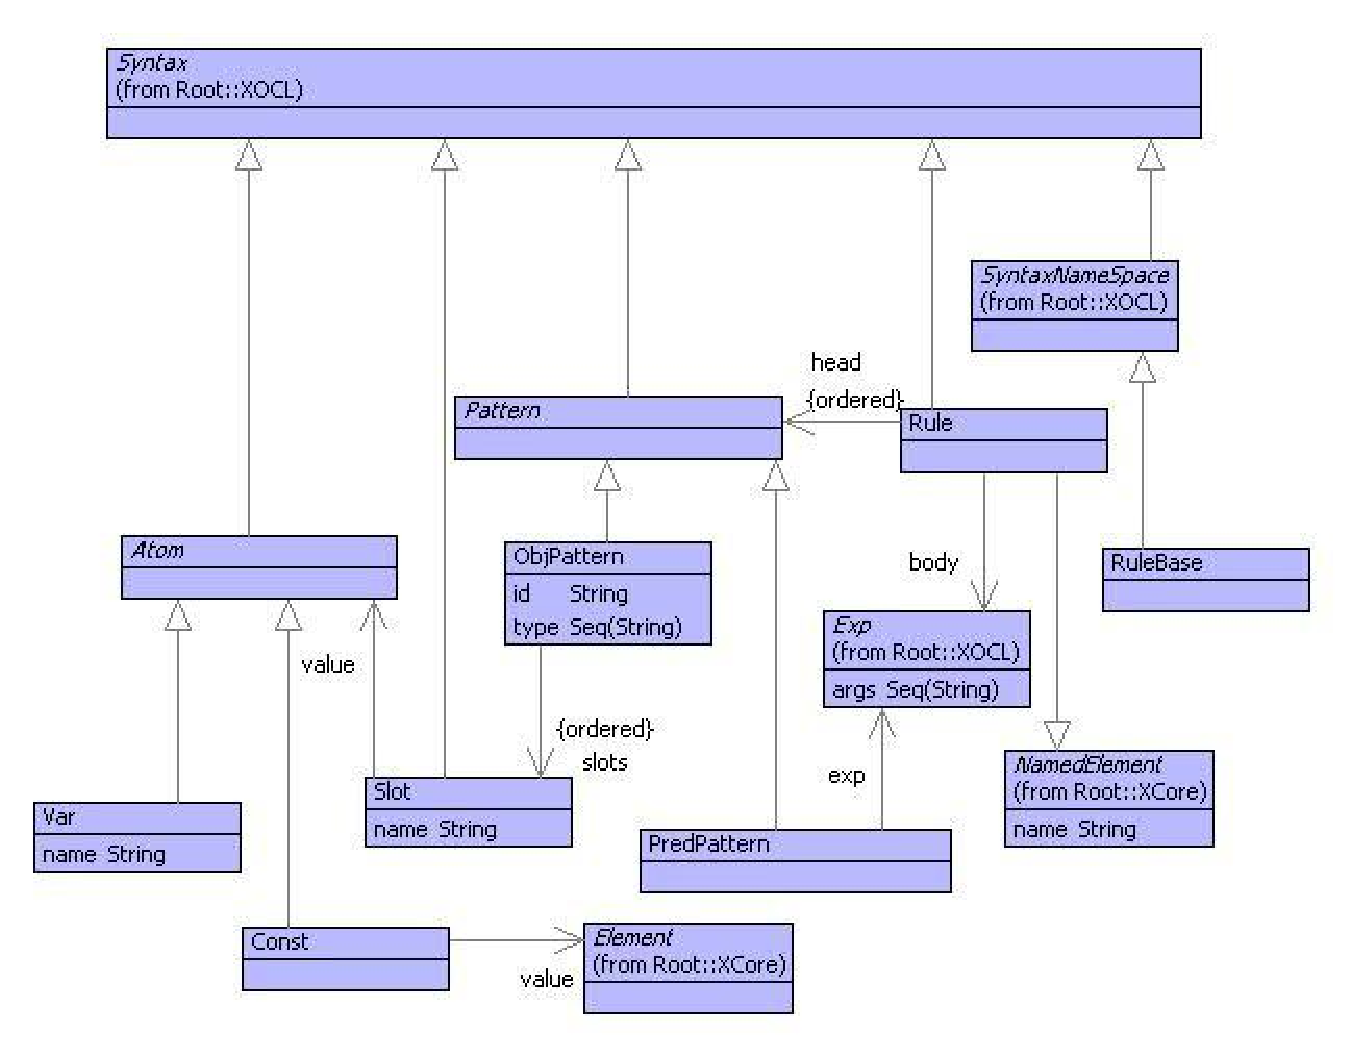
\includegraphics[width=12cm]{LanguageEngineering/BizRules/Images/Rules}

\caption{Business Rules Model\label{fig:Business-Rules-Model}}

\end{center}
\end{figure}


The first step in implementing the business rules engine describes
in the previous section is to construct some syntax classes and a
grammar that synthesizes the rules. Figure \ref{fig:Business-Rules-Model}
shows the model of the business rules syntax. All the classes in the
model inherit from XOCL::Syntax so that instances of the classes evaluate
to themselves (i.e. there is no evaluation phase-shift). The class
RuleBase is a name-space for rules; name-spaces are special and inherit
from SyntaxNameSpace. Each rule is a named element and has a head
and a body. Each element of the rule-head is a pattern: either an
object pattern or a predicate pattern. An object pattern references
a type by giving its absolute path as a sequence of strings. An object
pattern has an id that names an oject that matches the pattern. Each
slot of an object pattern has a name and an atomic value; the atomic
value is either a variable or a constant. 

A predicate pattern is an expression. The free variables of the predicate
are encoded as arguments of the expression. This makes it easy to
supply the values of the free variables to the expression when it
is evaluated. The body of a rule is also an expression. 

The rest of this section describes the grammar that translates from
concrete rule-base syntax to instances of the rule-base classes described
above.

A rule-base is a name-space and as such contains a collection of sub-expressions
each of which are added to the rule-base:

\begin{lstlisting}
@Grammar extends OCL::OCL.grammar
  RuleBase ::= name = Name rules = Exp* 'end' {
    rules->iterate(r rb = RuleBase(name) | rb.add(r))
  }.
end
\end{lstlisting}The syntax for rules is defined separately from that of rule-bases.
A rule is defined in isolation and is then added to the rule-base
either as part of the rule-base definition or via a context definition.
The grammar definition for Rule is straightforward except for the
use of XOCL::Exp to encode the predicate patterns and the rule-bodies.
Note how the FV operation of Performable is used to calcuate the free
variables referenced in an expression and set them as the arguments
of the operation that implements the expression:

\begin{lstlisting}
@Grammar extends OCL::OCL.grammar
  Rule ::= 
    name = Name 
    patterns = RulePattern* '->' exp = Exp 'end' {
      Rule(name,patterns,Exp(exp,exp.FV()->asSeq,null))
  }.
  RulePattern ::= 
    ObjPattern 
  | PredPattern.
  PredPattern ::= '?' exp = Exp 'end' { 
    PredPattern(Exp(exp,exp.FV()->asSeq,null)) 
  }.
  ObjPattern ::= 
    type = PType '[' id = Name slots = (',' Slot)* ']' {
      ObjPattern(type,id,slots)
  }.
  PType ::= n = Name ns = ('::' Name)* { Seq{n | ns} }.
  Slot ::= name = Name '=' a = SlotValue { Slot(name,a) }.
  SlotValue ::= 
    n = Name { Var(n) } 
  | s = Str { Const(s) } 
  | i = Int { Const(i) } 
  | 'true' { Const(true) } 
  | 'false' { Const(false) }.
end
\end{lstlisting}
\section{Rete Networks}

%
\begin{figure}
\begin{center}

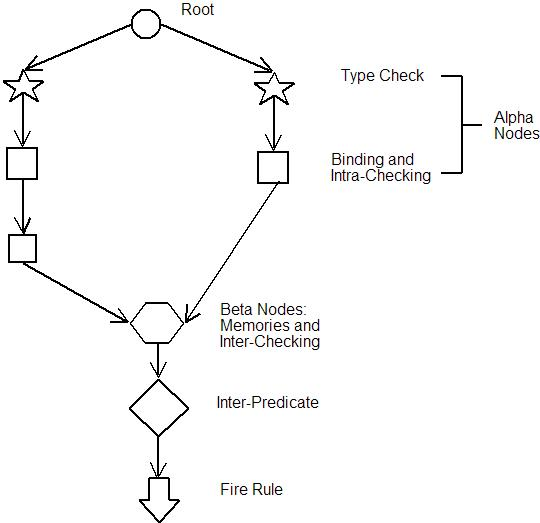
\includegraphics[width=12cm]{LanguageEngineering/BizRules/Images/Network}

\caption{A Rete-Network Fragment\label{fig:A-Rete-Network-Fragment}}

\end{center}
\end{figure}


A naive implementation of business rules would use an engine that
applies all business rules to all business data each time an event
occurs. Unfortunately, the performance of such an engine would not
be acceptable. Each rule typically involves matching and combining
multiple data elements. Each head pattern may contain multiple object
patterns. Each object pattern may match many different data elements
and a rule will become enabled for each combination of matching elements.
As the numbers of data elements increase, the number of combinations
that cause a rule to become enabled rises dramatically. If all combinations
must be checked and re-checked for each change in the business data
then the performance of rule matching will quickly become unacceptable.

The Rete Network matching algorithm was developed to address this
problem. It caches partial rule matches so that when a business event
occurs, only rule matching activities involving the changed data are
necessary. No matching involving unchanged data needs to take place.
This leads to a rule matching engine that can accommodate very large
number of rules and business data.

To see how the matching algorithm works, consider a simple rule:

\begin{lstlisting}
@Rule Example
  C1[c1,s1=v]
  C2[c2,s2=s1,s3=w]
  ? v > w end
-> e
end
\end{lstlisting}
The example rule matches any number of C1 and C2 instances such that
c2.s2 = c1.s1 and where c1.s1 > c2.s3. Rete proceeds as follows: all
new instances of C1 match the first pattern and are stored in the
rule memory. All new instance of C2 match the second pattern (ignoring
the s2 consistency issue), these are also stored in the rule memory.
The two parts of the rule memory are referred to as left and right
(C1 and C2 instances). 

As soon as a change occurs that leads to elements in both left and
right memories, the rule then matches the most recent entry with all
elements in the other memory. If a c1 is added to the left memory
then it is compared with element elements in the right memory; if
a c2 is added to the right memory then it is compared to all elements
in the left memory. Comparison checks for slot consistency: c2.s2
= c1.s1. For each pair that passes the consistency test, the algorithm
contines with the match.

Combined pairs of C1 and C2 instances are then filtered by the predicate
pattern v > w where v is a slot from the left-memory element and w
is from the right-memory element. If the predicate is astified then
the pair passes through and, since there is nothing left to check
, the rule is enabled. An enabled rule is added to the \emph{conflict
set}. If there is a non-empty conflict set then a rule is selected
(using a suitable choice algorithm) and its body is performed with
respect to the pair of C1 and C2 instances.

The structure of a Rete Network for Example is given in figure \ref{fig:A-Rete-Network-Fragment}.
A new or changed data element is supplied to the network root node.
The root node feeds the element to test nodes that check the type
of the element. In the case of Example, the types are C1 and C2 respectively.
If the type checks pass then the elements are passed on to \emph{alpha-nodes}
that check the internal consistency of the data and bind any variables.
In the case of Example, C1 requires a single alpha-node to match s1,
C2 requires two alpha nodes to match s2 and s3. 

Alpha nodes then feed into the left and right memories of a \emph{beta-node}.
A beta-node is responsible for pairing up matching data from the left
and right and performing inter-data checks. Once the beta-nodes are
satisfied they pass the data on to inter-element predicate nodes and
then on to nodes that fire rules into the conflict set.

Rules may have more patterns than Example given above. In this case,
for each object pattern pairing, the rule will have a pair of left
and right memories to store matching elements. The rest of this section
describes an executable model for Rete Networks.

%
\begin{figure}
\begin{center}

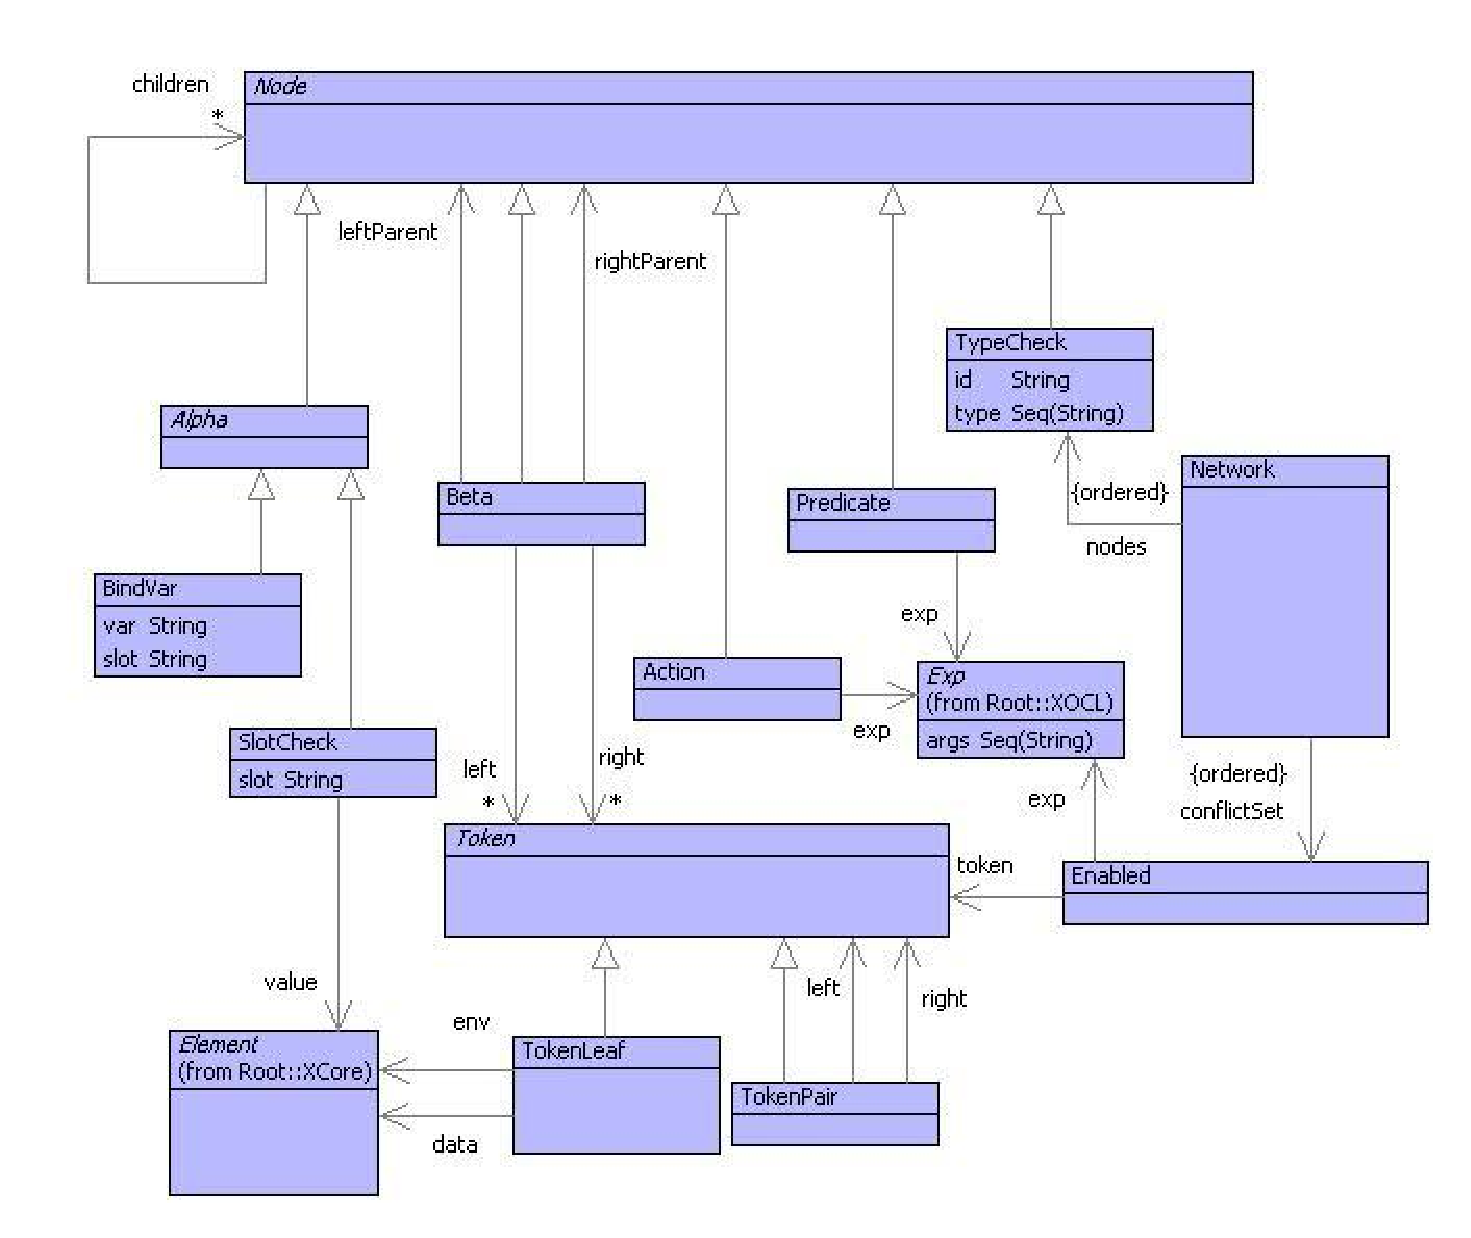
\includegraphics[width=12cm]{LanguageEngineering/BizRules/Images/Networks}

\caption{Rete Network Model\label{fig:Rete-Network-Model}}

\end{center}
\end{figure}


Figure \ref{fig:Rete-Network-Model} shows the model for a Rete Network.
A network consists of a collection of type checking nodes and a collection
of enabled rules. The rest of the network consists of nodes of different
types, all of which have 0 or more children.

Alpha nodes are either binding nodes or slot checking nodes. Predicate
and action nodes use expressions to represent executable predicates
and rule bodies respectively. Beta nodes have a left and right memory.

Tokens contain data elements to be matched by the network. A token
is either a single element of data (TokenLeaf) together with an environment
that binds rule variables with slot values, or a combination of two
tokens (TokenPair). The idea is that a leaf is initially added to
the network; each time the token is combined via a beta-node, the
tokens from the left and right memories are conmbined to become token
pairs. After several combinations, a rule is fired into the conflict
set together with a tree of tokens.

\begin{lstlisting}
context Network
  @Operation add(value)
    @For node in nodes do
      node.add(TokenLeaf(value,Seq{}),self)
    end
  end
\end{lstlisting}\begin{lstlisting}
context TypeCheck
  @Operation add(token,network)
    if token.data().isKindOf(type->lookup)
    then 
      @For node in children do
        node.add(token.bind(id,token.data()),self,network)
      end
    end
  end  
\end{lstlisting}\begin{lstlisting}
context SlotCheck
  @Operation add(token,parent,network)
    if token.data().hasSlot(slot) andthen
       token.data().get(slot) = value
    then
      @For node in children do
        node.add(token,self,network)
      end
    end
  end
\end{lstlisting}\begin{lstlisting}
context BindVar
  @Operation add(token,parent,network)
    if token.data().hasSlot(slot)
    then
      @For node in children do
        node.add(token.bind(var,token.data().get(slot)),self,network)
      end
    end
  end
\end{lstlisting}\begin{lstlisting}
context Beta
  @Operation add(token,parent when parent = leftParent,network)
     self.addToLeft(token);
     @For rightToken in right do
       let token = token + rightToken
       in if token.consistent()
          then 
            @For node in children do
              node.add(token,self,network)
            end
          end 
       end
     end
   end
\end{lstlisting}\begin{lstlisting}
context Predicate
  @Operation add(token,parent,network)
    let args = exp.args->collect(a | self.lookup(a,token))
    in if exp.op.invoke(network,args)
       then super(token,parent,network)
       end
    end
  end
\end{lstlisting}\begin{lstlisting}
context Action
  @Operation add(token,parent,network)
    network.addToConflictSet(Enabled(token,exp))
  end
\end{lstlisting}
\section{Rule Compilation}

Rules are compiled into a network by translating each of the head
patterns into sequences of alpha nodes and then combining the patterns
using beta-nodes. Compilation of a rule-base is supplied with a network.
The compiler updates the network with all the rules:

\begin{lstlisting}
context RuleBase
  @Operation compile(network)
    @For rule in self.contentsOf(Rule) do
      rule.compile(network)
    end;
    network
  end
\end{lstlisting}A rule consists of a head and a body. The head consists of a sequence
of patterns; each pattern may be an object pattern or a predicate
pattern. The object patterns are compiled first. Each object pattern
is of the form C{[}s1,s2,...,sn] where C is a classifier and each
si is a slot. An object pattern is compiled into a sequence of nodes
that test properties of tokens that are added to the network. The
nodes must check that the token has an object of type C and then must
check each of the slots of the token. Each slot must match each of
the slots si in turn: of the slot requires a variable to be bound
then the token is extended with a binding for the variable. if the
slot requires the object to have a particular slot value then the
token is checked, if the token's object does not have the required
slot value then the token is discarded.

If a rule head contains a sequence of object patterns then they are
compiled and the resulting sequences of nodes are combined pair-wise
using beta-nodes. The beta-nodes merge the tokens that match the two
object patterns. Beta-nodes are also responsible for checking the
consistency of bindings for repeated variable occurrences.

Finally, after each of the object patterns have been added to the
network and merged using beta-nodes, the predicate patterns are compiled.
Each predicate pattern produces a node that is supplied with a token.
If the predicate is satisfied by the data and environment in the token
then the token is passed on otherwise it is discarded:

\begin{lstlisting}
context Rule
  @Operation compile(network)
    let oPatterns = head->select(p | p.isKindOf(ObjPattern));
        pPatterns = head->select(p | p.isKindOf(PredPattern))
    in pPatterns->iterate(p node = self.compilePatterns(oPatterns,network) |
         let newNode = p.compile()
         in node.addToChildren(newNode); 
            newNode
         end).addToChildren(Action(body))
    end
  end
context Rule
  @Operation compilePatterns(Seq{pattern},network)
    pattern.compile(network)
  end
context Rule
  @Operation compilePatterns(Seq{pattern | patterns},network)
    pattern.compile(network)
      .join(self.compilePatterns(patterns,network))
  end
\end{lstlisting}Nodes are joined together as follows:

\begin{lstlisting}
context Node
  @Operation join(node when node.isKindOf(Predicate))
    self.addToChildren(node);
    node
  end
context Node
  @Operation join(node)
    let beta = Beta(self,node)
    in self.addToChildren(beta);
       node.addToChildren(beta);
       beta
    end
  end
\end{lstlisting}A predicate pattern is compiled to become a predicate node:

\begin{lstlisting}
context PredPattern
  @Operation compile()
    Predicate(exp)
  end
\end{lstlisting}An object pattern is compiled into a type checking node followed by
a sequence of slot checking nodes:

\begin{lstlisting}
context ObjPattern
  @Operation compile(network)
    self.compileSlots(slots,network.typeCheck(type,id))
  end
context ObjPattern
  @Operation compileSlots(Seq{},node) 
    node 
  end
context ObjPattern
  @Operation compileSlots(Seq{slot | slots},node)
    let newNode = slot.compile()
    in node.addToChildren(newNode);
       self.compileSlots(slots,newNode)
    end
  end
\end{lstlisting}An object pattern requires that the type of the data in a token is
checked. A TypeCheck node is added to the network. When a token is
received by a type check node, the type of the token data is checked.
If the type matches the required classifier then the token passes
on otherwise it is discarded:

\begin{lstlisting}
context Network
  @Operation typeCheck(type,id)
    @Find(node,nodes)
      when node.type() = type
      else 
        let node = TypeCheck(type,id)
        in self.addToNodes(node);
           node
        end
    end
  end
\end{lstlisting}Slots are compiled to become nodes that bind variable or check the
values in slots:

\begin{lstlisting}
context Slot
  @Operation compile()
    value.compile(name)
  end
context Var
  @Operation compile(slot)
    BindVar(slot,name)
  end
context Const
  @Operation compile(slot)
    SlotCheck(slot,value)
  end
\end{lstlisting}The following rule-base:

\begin{lstlisting}
@RuleBase Test
  @Rule r1
    C[c,slot1=v,slot2=100]
    D[d,slot3=v]
    ? v > 10 end
  ->
    e
  end
end
\end{lstlisting}is compiled by Test.compile(Network()) to produce the following network:

\begin{lstlisting}
Network[
  conflictSet = Seq{},
  nodes =
    Seq{
      TypeCheck[
        type = Seq{D},
        id = d,
        children =
          Set{
            #(3)=BindVar[
              slot = slot3,
              var = v,
              children =
                Set{#(4)=Beta[
                      left = Set{},
                      right = Set{},
                      leftParent = #(5)=SlotCheck[
                                     slot = slot2,
                                     value = 100,
                                     children = Set{#(4)}],
                      rightParent = #(3),
                      children =
                        Set{Predicate[
                              exp = [| v > 10 |],
                              children =
                                Set{Action[
                                      exp =
                                        [| e |],
                                      children = Set{}]}]}]}]}],
      TypeCheck[
        type = Seq{C},
        id = c,
        children = Set{BindVar[
                         slot = slot1,
                         var = v,
                         children = Set{#(5)}]}]}]
\end{lstlisting}
\section{Network Execution}

Once compiled, the network is used to implement the rules. When an
object is created it is added to the network. The state of the object
is recorded in the network in order to maximise the speed of multipl
object matching. When an object changes, the object is removed from
the network and then re-introduced. This section describes how the
network executes in terms of adding and removing objects.

Objects are added to a network as tokens. The token allows the engine
to manage the object along with any variable bindings that have been
associated with it during the match:

\begin{lstlisting}
@Class Token isabstract 
  @Operation add(other:Token):Token
    TokenPair(self,other)
  end
  @Operation consistent()
    // Repeated use of variables have the same values...
    self.env()->forAll(b1 |
      self.env()->forAll(b2 |
        b1->head = b2->head implies b1->tail = b2->tail))
  end
  @AbstractOp env():Seq(Element)
  end
  @AbstractOp lookup(name:String)
    // Look up the supplied variable name
  end
end
\end{lstlisting}When an object is introduced to the network, a leaf-token is created
to contain and manage it. The class LeafToken is a sub-class of Token
that uses an environment to lookup the supplied variable name. Two
tokens are merged on the output of a beta-node. Two tokens are merged
to produce a single token as an instance of TokenPair which is a sub-class
of Token and just contains two component token instances. The token-pair
implements lookup by delegating to the two component tokens.

An object is added to the network as follows:

\begin{lstlisting}
context Network
  @Operation add(value)
    @For node in nodes do
      node.add(TokenLeaf(value,Seq{}),self)
    end;
    self
  end
\end{lstlisting}In general, a node just passes a token on to its children:

\begin{lstlisting}
context Node
  @Operation add(token,parent,network)
    @For node in children do
      node.add(token,self,network)
    end
  end
\end{lstlisting}One of the first inodes in a network is a type-check node that filters
out objects by type:

\begin{lstlisting}
context TypeCheck
  @Operation add(token,network)
    if token.data().isKindOf(type->lookup)
    then 
      @For node in children do
        node.add(token.bind(id,token.data()),self,network)
      end
    end
  end
\end{lstlisting}Once an object has been determined to be of the required type it must
pass all the alpha-node checks before joining beta-memories and possibly
firing rules into the conflict set. Each rule may involve slot-checks:

\begin{lstlisting}
context SlotCheck
  @Operation add(token,parent,network)
    if token.data().hasSlot(slot) andthen
       token.data().get(slot) = value
    then
      @For node in children do
        node.add(token,self,network)
      end
    end
  end
\end{lstlisting}If the rule specifies that the slot value is just a variable then
the following node is used to bind the variable:

\begin{lstlisting}
context BindVar
  @Operation add(token,parent,network)
    if token.data().hasSlot(slot)
    then
      @For node in children do
        node.add(token.bind(var,token.data().get(slot)),self,network)
      end
    end
  end
\end{lstlisting}A predicate node is used to check an arbitrary boolean expression
using the values of varaibles that have been bound at that point in
the match:

\begin{lstlisting}
context Predicate
  @Operation add(token,parent,network)
    let args = exp.args->collect(a | self.lookup(a,token))
    in if exp.op.invoke(network,args)
       then super(token,parent,network)
       end
    end
  end
\end{lstlisting}That concludes the alpha-nodes. Next we must deal with the inter-clause
and inter-rule matching. This is handles by beta-nodes. The behaviour
of a beta-nodes when a token is added depends on whether the token
arrives form the left or the right. This is tested by defining two
'add' operations in BetaNode that use guards on the operation arguments
comparing the supplied parent with the left and right parent of the
node:

\begin{lstlisting}
context BetaNode
  @Operation add(token,parent when parent = leftParent,network)
    self.addToLeft(token);
    @For rightToken in right do
      let token = token + rightToken
      in if token.consistent()
         then 
           @For node in children do
             node.add(token,self,network)
           end
         end 
      end
    end
  end
context BetaNode
  @Operation add(token,parent when parent = rightParent,network)
    self.addToRight(token);
    @For leftToken in left do
      let token = leftToken + token
      in if token.consistent()
         then 
           @For node in children do
            node.add(token,self,network)
           end
         end
      end
    end
  end
\end{lstlisting}If a token ever reaches an action node then it has enabled a rule
and the rule is added to the conflict set of the network:

\begin{lstlisting}
context Action
  @Operation add(token,parent,network)
    network.addToConflictSet(Enabled(token,exp))
  end
\end{lstlisting}The network implements a remove operation that performs the same function
as add defined above, except that the tokens are removed from the
beta-memories when they arrive at beta-nodes and also removed from
the conflict set of the rule becomes enabled.


\section{Monitoring Classes}

In order to complete the implementation of business rules we require
that newly created objects are added to the network and when the object's
state is updated, they are removed and then re-inserted into the network.
To do this automatically we implement a new-meta-class that manages
instances appropriately:

\begin{lstlisting}
import Daemon;

context Root
  @Class MonitoredClass extends Class
    // Classes whose instances are to be monitored by a
    // rule-based that has been compiled into a network
    // should be instances of the meta-class MonitoredClass.
    @Bind daemon =
      // The following daemon is added to all new instances
      // of monitored classes. The daemon ensures that all
      // changes to the object cause the network to be
      // informed via add and remove...
      Daemon("MonitorDaemon",ANY,
        @Operation(object,slot,new,old)
          object.of().network().remove(object);
          object.of().network().add(object)
        end)
    end
    
    // Each monitored-class must specify which network is
    // to be used for its instances...
    @Attribute network : Network (?,!) end   
    
    @Operation add(element)
      // The network for a monitored-class can be
      // specified in the definition of the class
      // and added to the class via this operation...
      @TypeCase(element)
        Network do
          self.network := element
        end
        else super(element)
      end
    end
    
    @Operation invoke(this,args)
      // By defining an invoke operation we hi-jack the
      // class instantiation process for a monitored-class.
      // The new instance is created in the usual way but
      // the daemon is added to the object before it is returned 
      // and the new object is added to the network...
      let newObj = super(this,args)
      in newObj.addDaemon(MonitoredClass::daemon);
         network.add(newObj);
         newObj
      end
    end
  end
\end{lstlisting}
